% Capítulo 4
\chapter{Taxonomia}
\label{cap:cap4}

Seguindo a análise dos trabalhos mencionados no Capítulo \ref{cap:cap3}, verifica-se a necessidade de classificar dos conceitos mais recorrentes atrelados ao uso do padrão \textit{throttling} em redes IoT com dirigidas energética. Além disso, é preciso levar em consideração a orientação do trabalho junto aos critérios de disponibilidade definidos por \cite{avizienis_basic_2004}, base para categorização dos elementos propostos nesta taxonomia. 

\section{Organização}

Inicialmente, as classes foram distribuídos acomodando os elementos envolvidos de acordo com os critérios que os definem, a seguir, conforme apresenta a Figura \ref{fig:taxonomia_geral}.


\begin{figure}[h]
\noindent\includegraphics[width=3cm]{example-image} 
\caption{Aqui vou colocar uma figura apresentando os dois grupos da taxonomia}
\label{fig:taxonomia_geral}
\centering
\end{figure}

Nas ramificações à esquerda, encontram-se categorias que representam as características principais relacionadas aos elementos presentes em ambientes \acf{IoT} com restrições significativas de energia. Em \cite{kansal_power_2007}  percebeu-se a necessidade de classificar estes elementos como pertencentes a uma relação de compartilhamento dos recursos disponíveis, sensores, atuadores e até mesmo os energéticos. Para isto, na taxonomia de \cite{avizienis_basic_2004} há uma divisão clara entre os agentes envolvidos e sua natureza em dois agrupamentos principais: um grupo denominado usuários ou clientes, que atua ativamente ou de forma passiva solicitando recursos ou quando notificado, consumindo os estados ofertados do segundo grupo, os provedores. Aos nodes provedores, cabe a responsabilidade de compartilhar seus recursos com os nodes consumidores através de uma interface conhecida de acordo com o protocolo de comunicação pré-estabelecido entre as partes.

Toda interação deve seguir um padrão de operação, esta é realizada de acordo com o qual se destina, como visto no trabalho de \cite{khairnar_discrete-rate_2015} é apresentado uma operação como a medida pelas quais mensagens são trocadas entre nodes para um determinado fim. Sendo assim, os elementos classificadores encontrados são: \textit{Agentes}, \textit{Recursos} e \textit{Operações}.

Ademais, à direita, acomoda-se os elementos envolvidos no processo de adequação do comportamento da de um node através da adoção do padrão \textit{Throttling}. Nesta, dois ramos principais são apresentados, \textit{Atuação} e \textit{Implementação} respectivamente. Sobre \textit{Atuação}, agrupa-se os elementos envolvidos no processo de controle do consumo dos recursos do node: \textit{Limiar} - \textit{Thresholding}, \textit{Ciclos de Carga} e \textit{Meios} estado diretamente relacionados à ação de limitar a taxa de resposta dos serviços,  \cite{khairnar_discrete-rate_2015}, \cite{khan_energy_2015} e \cite{sudevalayam_energy_2011} abordam questões que podem particularmente serem observadas para os elementos orientados energeticamente. A \textit{Implementação} é sugerida de maneira à assegurar que os critérios  \textit{Observáveis} e seus \textit{Motivadores} sejam agentes orientadores no processo de restrição às operações e incremento da disponibilidade do node. 


\section{Taxonomia Proposta}
A Figura apresenta em resumo a taxonomia proposta e os pontos abordados no processo de uso do padrão \textit{throttling} como alternativa para garantir disponibilidade nos nodes presentes em uma rede \acs{IoT} dirigida a energia. O objetivo principal é dispor os elementos ligados ao tema de maneira visual e contemplar a organização dos tópicos envolvidos. Com isso, obter:

\begin{enumerate}
    \item Visão sobre os elementos envolvidos em uma rede \acs{IoT} dirigida a energia e apresentar o \textit{Throttling} como mecanismo regulador do comportamento observando suas características energéticas;
    \item Organizar as classes de conhecimento relacionadas acomodando-as de acordo com o contexto de inserção;
    \item Suporte às definições de uso do padrão \textit{Throttling} ligados ao contexto de redes \acs{IoT} dirigida a energia. 
\end{enumerate}

\begin{figure}[h]
\noindent\includegraphics[width=3cm]{example-image} 
\caption{Aqui vou colocar uma figura da taxonomia proposta}
\label{fig:taxonomia_detalhada}
\centering
\end{figure}

A taxonomia detalhada apresenta suas classes nos termos em que foram encontrados na literatura dentro contexto de estudo, conforme Figura \ref{fig:taxonomia_detalhada}.

\section{Agentes \acs{IoT}}
Cada agente é essencialmente uma entidade que tem a capacidade intrínseca de interagir com outros agentes digitais ou físicos. Eles possuem propriedades fundamentais, como funcionalidade, desempenho, confiabilidade e segurança \cite{avizienis_basic_2004}. No contexto da Internet das Coisas (IoT), é crucial considerar sua capacidade de se comunicar com outras entidades, atuando em conjunto através do compartilhamento de recursos, características embarcadas nos dispositivos \cite{asghari_internet_2019}.


\subsection{Node Provedor}

Em qualquer instância em que um node computacional oferece um estado ou responde a uma solicitação de recurso, ele assume o papel de provedor. Geralmente, um node desse tipo pode oferecer uma ou mais funcionalidades por meio de serviços, cada uma sendo atendida pelo uso de seus recursos enquanto avança em seus estados internos em busca de fornecer uma resposta à interação. O resultado disto será percebido como  estado externo, acessível por meio de uma interface provida na forma de eventos ou como resposta às solicitações motivadores por meio de nodes clientes. 

Um Serviço, representa ao node provedor a maneira como o mesmo lida com seus recursos embarcados. Estes serviços motivam a dinâmica de mudanças de estado internos.  Por exemplo, tomemos um sistema de iluminação publica que solicita a seus dispositivos alimentados por baterias e dispostos em um ambiente, para que acionem um recurso do tipo lampada em razão da detecção de movimento no mesmo ambiente onde o node provedor está inserido. Tal ação é ofertada  via serviço que por sua vez impactará em algum desgaste da lambada bem como a depreciação de seus recursos energéticos.

\begin{figure}[H]
	\centering
	\caption{Representação de Node Provedor.}
	\label{fig:cap4nodeprovedor}
	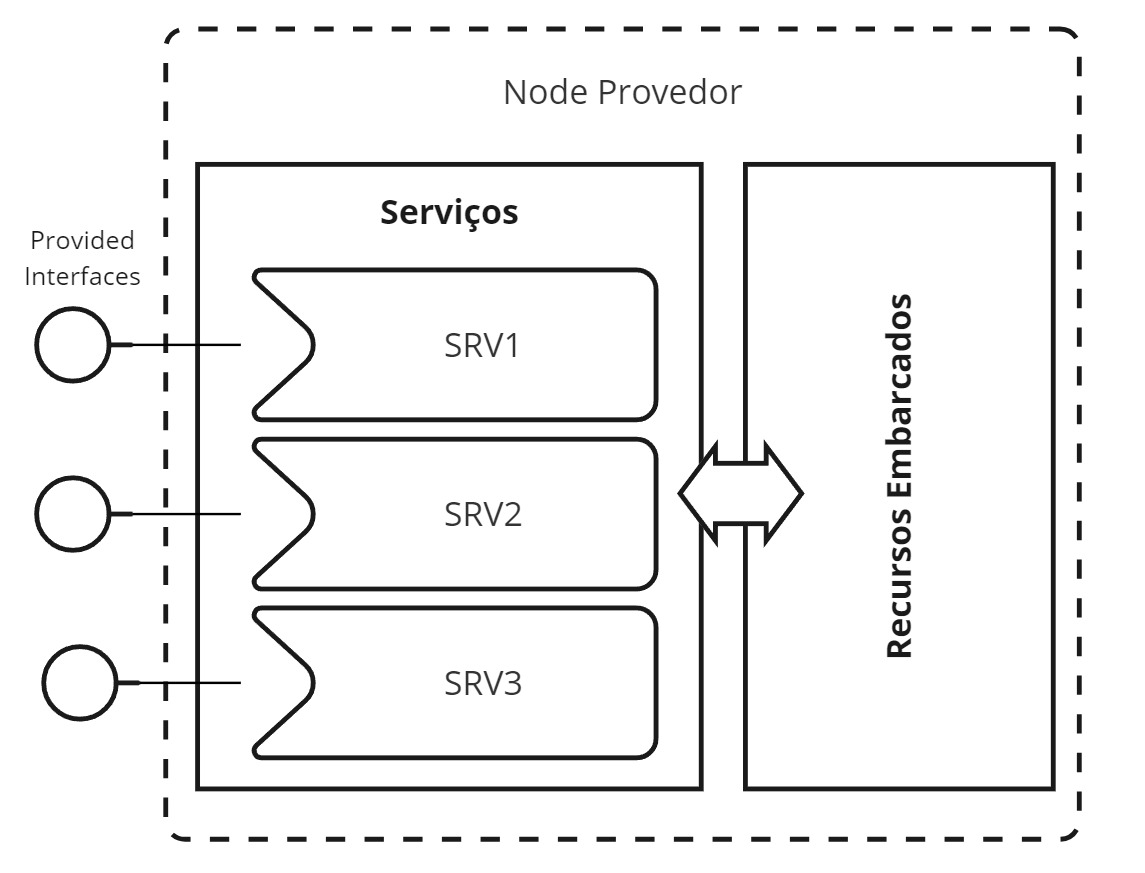
\includegraphics[width=0.7\linewidth]{Imagens/cap4/cap4nodeprovedor}	
	
	Fonte: elaborado pelo autor.
\end{figure}

\subsection{Node Cliente}
Um node cliente é responsável por receber o estado externo de nodes provedores por meio de uma interface disponibilizada. Ele pode consumir recursos de um ou mais provedores, dependendo da operação em execução. O node cliente comunica-se com os provedores necessários para realizar suas operações, de acordo com suas particularidades. Tal dinâmica representada na Figura 

\section{Operações}
Operações consiste no fluxo de mensagens comunicáveis entre nodes clientes e provedores. Uma operação é realizada quando um cliente através de mensagens solicita estado de um provedor, de outra maneira, também é possível um provedor ativamente disponibilizar um estado, dito externo para que um possível cliente possa utiliza-lo. 

Mensagem é a unidade atômica de informação que independente do seu formato é utilizada para as mais diversas ações de acordo com o que se destina a rede colaborativa, uma mensagem pode carregar ações como  inicialização, controle, monitoramento, coleta, processamento ou armazenamento de dados. A depender da funcionalidade, um cliente quando ativo, deve enviar mensagens de solicitação aos provedores os quais reativamente respondem via interface preestabelecida, caso a operação aconteça através de eventos, o provedor deve autonomamente disponibilizará suas informações para todos que tenham interesse.

Para cobrir uma operação, múltiplas mensagens podem ser solicitadas na forma de composição de serviço \cite{service_composition}, nesse cenário um node cliente solicita mensagens distintas à um ou vários nodes provedores para compor este serviço. Em todo caso, como encontrado na revisão \cite{kahloul_service_2019} a abordagem das operações encontrada nos serviços puramente virtuais não acomodam por completo a natureza operacional dos agentes \acp{IoT}. Para tal, precisa-se considerar o estado dos nodes e seus recursos pois estes se encontram diretamente em um meio físico e precisam lidar com as particularidades inerentes a um ambiente dinâmico e seus desafios.

\section{Recursos Energéticos}

Um Recurso descreve um componente ou capacidade que um dado node possui para realizar suas operações. Isto inclui seus componentes físicos ou virtuais que uma vez embarcados ao dispositivo contribuem em cooperação para os mais diversos fins, coleta, monitoramento, automação industrial, assistência a medicina entre outros. Um Recurso infere sobre as capacidades dos elementos dispostos na rede, a configuração do dispositivo esta fortemente ligado à atividade fim que se destina. Para este trabalho, os recursos como processamento, armazenamento ou capacidade de transmissão estão omitidos pois expressam diretamente o universo de possibilidades onde um agente \acs{IoT} se encontra. Entretanto, em uma rede \acp{IoT} dirigida à energia, aspectos energéticos devem ser detalhados

Recursos energéticos refere-se a dois grupos: da capacidade de coleta do node e a capacidade de armazenamento e disponibilização da energia previamente coletada. Arquitetura de sistemas dirigidos a energia com capacidade de coleta são projetados para usar estes recursos de maneira eficiente como descrito em \cite{prauzek_energy_2018} sua aplicação é especialmente útil em cenários onde a energia para alimentar os componentes eletrônicos é escassa. Um recurso energético é propriamente uma fonte natural ou artificial de energia que de maneira apropriada pode ser convertida em energia utilizável para garantir a realização das operações. 

No cenário proposto, assume um papel importante pois é essencial para garantir o funcionamento continuo e autônomo dos nodes envolvidos, cabendo ao agente suas ações de coleta, transformar, armazenamento e utilização o recurso energético, projetado de maneira a aproximar-se do estado onde as operações tendem a uma neutralidade energética \acfp{EN}, conceito apresentado por \cite{kansal_power_2007} e posteriormente em \cite{merrett_energy-driven_2017} com a abordagem da neutralidade de força-energética, em acordo com suas respectivas capacidades.

% \subsection{Sensores}
% Um sensor é um recurso capaz de detectar e medir informações específicas do ambiente ao redor. Convertendo características do meio físico como temperatura, umidade, luz, pressão, movimento, som em sinais digitais que podem ser processados. 

% \subsection{Atuadores}
% Por sua vez, um atuador é um componente que converte um sinal de entrada em um movimento físico ou ação. Em um sistema de controle um atuador pode receber uma entrada provida por um sensor e agir em detrimento do estimulo capturado.  Atuadores geralmente são categorizados em: elétricos, hidráulicos, pneumáticos, mecânicos (por exemplo, atuadores de engrenagens), magnéticos, piezoelétricos entre outros.





\subsection{Capacidade de Coleta}\label{Capacidade de Coleta}
De acordo com o trabalho de \cite{sudevalayam_energy_2011}, a capacidade de coleta refere-se à habilidade do elemento em extrair e transformar um recurso energético disponível no ambiente. Seu objetivo é manter ou estender o tempo de funcionamento do node, atendendo totalmente ou parcialmente às suas necessidades energéticas.

Sistemas de coleta energética possuem três conceitos fundamentais: Carga, a Arquitetura de Coleta e entrada energética. A Carga é destinada a atividade que esta consumindo energia, este é oriundo de um componente demandante de energia para operar, sejam sensores, transmissores ou  atuadores, apresentados como uma composição de recursos. A Arquitetura de Coleta indica quais mecanismos, deve descrever seus componentes, meios de conversão e unidades de armazenamento. Atualmente é possível destacar três modelos básicos de arquitetura:

\begin{itemize}
    \item Coleta e Usa (\textit{Harvest-Use}): Neste modelo, toda energia coletada é oferecida diretamente ao node continuamente. Conforme \cite{merrett_energy-driven_2017}, um node não precisaria de um \textit{buffer} energético, ou apenas o minimo possível para mante-lo operacional, desde que seu funcionamento for orientado as características da neutralidade força-energética. Assim, a energia coletada deve satisfazer os valores de operação plena ou pelo menos o minimo necessário para o funcionamento depreciado. Por isso, caso a energia coletada não seja suficiente, o node prontamente adaptará o fornecimento dos seus recursos buscando enquadrar-se a disponibilidade energética corrente para, posteriormente, caso o nível de fornecimento energético alcance os níveis desejados, tenha sua operação restabelecida. Em alguns casos, quando prontamente é detectado níveis energéticos abaixo do necessário até para o funcionamento adaptado no node, o mesmo, poderá executar alguma rotinas de \textit{checkpoint} para caso tenha sua operação integralmente interrompida, possa mediante ter sua necessidade energética suprida em momento futuro, retornar para um estado desejado, como sistemas intermitentes já mencionados em \cite{sliper_energy-driven_2020}.
    
	\begin{figure}[h]
			\centering
			\noindent\includegraphics[width=3cm]{example-image} 
			\caption{Aqui vou colocar uma figura power-neutral}	
	\end{figure}   
    
    \item Coleta, Armazena e Usa (\textit{Harvest-Store Use}): Dispositivos inseridos em um dado ambiente coletam energia do meio para seu uso. Todavia, estes nodes precisam lidar com o dinamismo da natureza energética coletada. Para tal, embarca-se ao node a capacidade de armazenar a energia coletada em um \textit{buffer} para posteriormente disponibilizar esta entrada para uso nos ciclos de carga do node. Este modelo visa contornar os dados problemas com variações em performance encontradas pelo \acs{EHS} seja pela depreciação do modelo de coleta ou até mesmo devido à escassez de energia disponível para coleta no meio em dado momento.
    
    \begin{figure}[h]
    	\centering
    	\noindent\includegraphics[width=3cm]{example-image} 
    	\caption{Aqui vou colocar uma figura energy-neutral}	
   	\end{figure}  
    
\end{itemize}


Sobre os ambientes onde nos nodes operam, diversas técnicas podem ser utilizadas para a extração de energia disponível, a conversão de energia renovável solar e eólica, a captura da força \textit{piezo-elétrica}, termodinâmica, entre outros. A adequação da estratégia de coleta e seus detalhes devem ser projetados de acordo com o meio onde node se encontra e a natureza da fonte energética que visa-se coletar. Em geral, a divisão das características dos ambientes já descrito em \cite{shaikh_energy_2016} pode ser utilizada para categoriza-las de acordo com seus ambientes, sendo assim se encontram em:

\begin{itemize}

    \item Não controladas mas previsíveis: A produção energética não pode ser controlada nos momentos desejados, mas o comportamento pode ser modelado para prever a disponibilidade num dado momento com alguma margem de acerto. Por exemplo, no trabalho de  \cite{lee_energy_2018} fontes energéticas baseadas em energia energia solar, que tem sua origem não controladas, todavia existem modelos capazes de prever  disponibilidade energética para colheita de acordo com sua sazonalidade durante ciclos diurnos.
    
    \item Não controladas e não previsíveis: A fonte energética não pode ser controlada para gerar energia quando desejado e não é fácil prever usando um modelo quando será possível. A extração energética originada pela vibração de ambientes internos é um exemplo de tal fonte energética como descrito em \cite{wei_comprehensive_2017}, todavia definir padrões de sazonalidade das vibrações pode tornar o processo de coleta impraticável;
    
    \item Completamente controlada: Neste contexto, a energia é gerada apenas quando necessário, como visto em alguns sistemas \textit{piezoelétrico} onde através da interação humana para geram energia quando necessário.
    
    \item Parcialmente controlada: O processo de geração energética é sensível à ação de terceiros porém a quantidade exata de energia gerada não pode ser prevista com exatidão. Fontes baseadas em Radio Frequência converte a transmissão de ondas de radio em energia utilizável, por exemplo, \cite{shaikh_energy_2016} decorre como tags \acf{RFID} conseguem ser visualizadas por um leitor. Todavia, a quantidade de energia coletada sofre impactos diretos das características de propagação no meio disposto, barreira, distancia até a fonte e capacidade da antena de transmissão.
\end{itemize}

\subsection{Capacidade de Armazenamento}\label{Capacidade de Armazenamento}
A capacidade de armazenamento trata de propriedades como conversão, força e taxa de carregamento e descarga em relação a fonte energética em uso com o objetivo de utilizar essa energia em momento apropriado. 

É bem conhecido que o fator energético é um desafio para redes com restrições energéticas e capacidade de coleta, pois claramente caso a energia de um node seja esgotada o mesmo não será capaz de cumprir seu papel a menos que o fornecimento energético seja restabelecido ou algum mecanismo de armazenamento possa cobrir parcial ou totalmente a diferença energética necessária para a operação.

Baterias, super capacitores ou modelos híbridos estão presentes no contexto de dispositivos com fortes restrições energéticas e capacidade de coleta, para estes a atuação busca estar de acordo com as condições físicas e necessidade de conservação da energia. É possível distinguir três padrões de armazenamento para as capacidade energética presente em um dispositivo que busca o estado de operação neutra onde se observa a relação entre a saída energética e o gasto energético do node dado o momento. Segundo o modelo de uso proposto, a habilidade para coleta e a necessidade de disponibilidade definida no \acs{SLA}, os nodes provedores encontram sua capacidade de armazenamento em um dos casos:

\begin{itemize}
    \item Node provedor sem reserva energética: Aqui não existe a necessidade estrita da gestão de recursos elétricos pois caso não exista energia suficiente o node irá adaptar-se na tentativa de alinhar a necessidade energética ao fornecido momentaneamente, em outros casos, sua operação se comportará como um sistema transiente, preparados para interromper suas atividades e, ao reestabelecer sua entrada energética disponível, retornar a partir de um ponto previamente estabelecido. Neste caso, é considerável existir uma pequena reserva, suficiente para conseguir armazenar um estado adequado ou ação semelhante.
    
    \item Node provedor com reserva energética: Neste caso, um node carrega em si a capacidade de armazenar energia coletada em um \textit{buffer}. A gestão energética deve ocorrer para que a energia coletada seja previamente armazenada para ai sim, ser disponibilizado em ciclos de carga. Aqui os nodes operam em um regime de Coleta, Armazenamento e Uso, já descrito anteriormente.
\end{itemize}

\section{\textit{Throttling}}

Aplicar o padrão \textit{Throttling} consiste basicamente em restringir o uso de recursos de acordo com limiares de utilização estabelecidos. Seu objetivo é proteger um dispositivo do estado de sobrecarga, evitando que consumidores excessivamente solicitantes coloquem um node provedor em um estado de sobrecarga, evitando possíveis falhas e a exaustão prematura de recursos \cite{martinekuan_throttling_nodate}. Com isso, a estratégia permite que provedores consigam operar dentro de termos definidos por um acordo de funcionamento conhecido como \acf{SLA}, protegendo este provedor de assumir um estado de sobrecarga onde precise atender mais solicitações do que o adequado para sua capacidade.

Na taxonomia, o uso do \textit{Throttling} é candidato à colaborar nas atividades que buscam aumentar disponibilidade do node provedor, conservando  recursos energéticos e suas observações a respeito de características ou limitações do próprio dispositivo. Para tal, é preciso que limiares sejam estritamente adequados ao que se aplica, capacidade de transmissão, recursos disponíveis ou esperados pelo node. Definir limiares de operação realísticos para o node provedor é um desafio relevante para sistemas com estratégia de coleta de energia \cite{khairnar_discrete-rate_2015}, \cite{liu_energy_2016} e \cite{zhang_toward_2018}, entregando capacidade de decisão sobre ciclos de carga enquanto se objetiva maximizar o tempo de vida do próprio node.

\subsection{Atuação: Limiar, Ciclo de Carga, Observáveis e Meios}
\label{cap4:atuação}
Em sistemas \acs{IoT} orientados aos fatores energéticos, a atuação do padrão é dada ao monitorar a taxa de solicitações no decorrer de um espaço de tempo, nesse intervalo, denominado Ciclo de Carga. Durante um ciclo nodes clientes podem fazer requisições ao provedor. Do ponto de vista da disponibilização dos recursos, durante um ciclo de carga, um node pode assumir abordagem de equidade entre os solicitantes ou algum critério de prioridade e privilégio, onde um solicitante qualquer teria suas requisições atendidas mediante negação do serviço para outro node cliente com menor prioridade, caso necessário.

Uma vez definido um limiar de atuação, sua ação pode ser inteiramente linear ou constante, onde durante todo funcionamento do node o mesmo valor limiar é aplicado, independente de outros fatores, outra possibilidade é definir vários limiares que agem adaptativamente de acordo com os diversos estados mapeados, tão logo determinado cenário seja alcançado, o node pode ajustar seu limiar de atuação para conservar seus recursos visando manter-se funcional. O comportamento do limiar de atuação passa pela analise cuidadosa da natureza do node provedor e operações esperadas. Em síntese:

\begin{itemize}
    \item Limiar constante: Seu valor é fixado e estabelecido enquanto o node é projetado. Este limiar pode ser determinado considerando fatores como testes de desempenho, características do ambiente onde será inserido e requisitos operacionais. Todavia, uma vez definido, o limiar permanecerá constante ao longo de todo o tempo das atividades do node. 
    
    Por exemplo, considere um node com uma dada capacidade de processar mensagens, este pode estabelecer um limiar constante para o máximo de requisições processáveis simultaneamente. Sendo assim, em toda operação, caso esse limiar de requisições seja atingido, o node irá ativamente optar por rejeitar ou atrasar o atendimento até que o valor de requisições retorne ao nível aceitado. 
    
    Esta abordagem, é bastante útil caso se conheça bem as capacidades do node e não se espera uma grande variação nas condições de operação ao longo do tempo. Embora oferte equidade do ponto de vista dos solicitantes (que tem suas requisições atendidas segundo os mesmos critérios independente do estado do node provedor), não se garante que uso dos recursos será adequado caso ocorra mudanças repentinas ou flutuações significativas nos termos de funcionamento deste provedor.
    
    \item Limiar adaptável: Nesta abordagem, o comportamento do node é ajustado dinamicamente, por isso um node pode assumir um comportamento mais adequado ao observar suas condições de funcionamento através do monitoramento ou auto-análise dos recursos do node, permitindo atender as solicitações dos nodes clientes, com performance adequada aos termos de operação que se encontre. Por exemplo, dado um sistema de segurança que geralmente possui nodes equipados com câmeras. Este provedor, deve enviar imagens capturadas por seus sensores para algum solicitante, seja uma central que passivamente recebe as gravações ou outra forma de node demandante. Dado uma mudança observada em seus termos de funcionamento, o node poderá ter faixas de limiares distintas adequando-se ao estado encontrado, conservando-se e garantido seu funcionamento dentro do \acs{SLA} estabelecido.   
    
    \begin{figure}[h]
    	\centering
    	\includegraphics[width=3cm]{example-image} 
    	\caption{Aqui vou colocar uma figura A e B com as diferentes atuações do limiar.}
    \end{figure}
    
    Graças a isso, o node com limiar adaptável será capaz de operar em diferentes faixas de operações, depreciando seus serviços com a mudança de comportamento, seja para interromper ou reduzir sua taxa da transmissão e assim permanecer operando mitigando riscos funcionais enquanto se encontre neste estado. Uma vez que os recursos observáveis se restabeleçam, o node pode assumir comportamento de uso acentuado dos recursos disponíveis permitido pelo novo valor estipulado para o limiar de consumo adequado. Esta capacidade de adaptação, permite que nodes provedores mantenham algum equilíbrio entre conservação de recursos e performance, garantindo suas funcionalidades nos termos das condições operacionais.
    
      
 
    
\end{itemize}


Ciclo de Carga, refere-se as atividades suportadas que consomem algum recurso energético do node dentro de um intervalo de tempo. Dado uma sistema com coleta de energia, um ciclo de carga durará pelo menos até que a próxima entrada energética coletada esteja disponível.  Uma carga é qualquer atividade que requer o consumo energético, seja sensoriamento, atuação, transmissão de dados entre outros. O mecanismo de \textit{throttling} irá atuar regulando o uso de recursos durante um ciclo, caso necessário, depreciando ativamente as operações de acordo com o projetado, visando adequar estas atividades de carga e o consumo energético ao cenário encontrado pelo provedor até que a próxima entrada energética esteja disponível e possa ser novamente adaptado em concordância com o novo cenário a que se encontra.

\begin{figure}[h]
	\centering
	\noindent\includegraphics[width=3cm]{example-image} 
	\caption{Aqui vou colocar uma figura sobre entrada energética e ciclo de carga.}
\end{figure}

Qualquer aspecto que impacte ou influencie na capacidade do node em manter-se disponível deve ser considerado em sua atuação. Estes, ditos elementos observáveis, compreendem os componentes aos quais cabem a analise de estado, pois justificam a ação do mecanismo throttling, que deverá indicar o comportamento do node para mante-lo adequado mediante evitar seu esgotamento energético. Para tal, se apresentam como os garantidores das condições energéticas do node: sua condição de entrada através de uma fonte energética; a capacidade de armazenamento dessa energia coletada em eventual \textit{buffer}. 

\subsubsection{Meios}
\label{cap4:atuacao_meios}
O comportamento de um node pode ser ajustado de acordo com as circunstâncias. Diferentes meios são usados no processo de aplicação de um mecanismo \textit{throttling} a depender da função do node na rede e a intenção particular ao limitar operações. Assim, os meios de atuação decorrem sobre:

\begin{enumerate}[label=(\subscript{Meio} {{\arabic*}})]
	\item \label{meio1} Atuação sobre nodes clientes; 
	\item \label{meio2} Atuação sobre atividades do node provedor;
	\item \label{meio3} Atuação sobre degradação intencional de componentes envolvidos.
\end{enumerate}

O \ref{meio1} usa de mecanismos de throttling ao considerar a necessidade de observar as capacidades dos nodes clientes em relação de sua taxa de vazão ou a criticidade de suas operações. Sobre a taxa de vazão, estipula-se um throttling aplicado a quando o node cliente buscar limitar sua taxa de recebimento de mensagens de acordo com sua capacidade de lidar com tais eventos. Sendo assim, para conseguir operar nos termos em que se encontrar, o node cliente poderá limitar sua vazão para envio ou recebimento de dados de acordo com as suas capacidades, este limite tem por objetivo recuperar ou preservar seus recursos em acordo com o estabelecido limiar de atuação.

Entende-se por criticidade de uma operação, o atributo que indica quão essencial é esta para o node. Sendo assim, sobre atuação do throttling nos nodes clientes, cabe dois cenários: um primeiro onde todas as operações tem igual importância para o node/rede, e um segundo, onde existam operações classificadas mais importantes que outras. Sendo assim, de acordo com o segundo cenário, justifica que tais operações possam encontrar alivio nos  limiares de throttling  e por isso, cabe observar e definir tais valores para que dado operações privilégiadas, exista também maior tolerância quanto ao uso de recursos para as tais. 

Certamente, para que seja possível um maior gasto de recursos pelas operações criticas, cabe também ao projeto definir regras de compensação onde o node poderá reduzir seu limiar para demandas menos criticas, caso necessário.

\ref{meio2} compreende o controle de atuação no node provedor. De acordo com o seu estado durante um ciclo de carga os mecanismos de throttling poderão atuar em conformidade aos recursos encontrados neste node. Para tal, as estratégias de aplicação e definição de limiares passam pela observação da capacidade de vazão das múltiplas solicitações proveniente dos clientes, bem como da criticidade das operações realizadas. 

A taxa de vazão do um node provedor, é definida pela sua capacidade em atender demandas dos diversos nodes solicitantes durante um espaço de tempo seja por limitação da rede ou por sua capacidade computacional em realizar tais operações. Sendo assim, o mecanismo de throttling poderá se valer dos limiares estipulados através da análise dos recursos disponibilizados para operação dentro da janela de tempo, a partir daí, dado o cenário encontrado, limitar o atendimento as solicitações de nodes considerados excessivamente demandantes ou menos privilégiados.  

Quanto a observação nas operações realizadas pelo node provedor, estas tem seu grau de criticidade atrelado a importância de tal operação na conjuntura ao qual se destina o node bem como quão fundamental pode ser. É importante destacar que a definição de limiares sempre busca garantir que o node não consuma seus recursos excessivamente, limiar este que deve ser revisto sempre que o panorama encontrado pelo node mude, seja pelo fim da janela de trabalho (carga) ou a medida que as atividades demandantes sejam atendidas. Com isso, dado limiar deverá atuar protegendo o node provedor no decorrer de suas trocas de estado a passo que realiza as operações. 

O limiar de atendimento de operações poderá suportar um sistema hierárquico, neste caso nodes solicitantes mais privilégiados terão suas operações realizadas mesmo em um cenário de escassez, outro ponto é que dado a criticidade da operação pode-se fazer distinção, tolerando mais operações de um tipo considerado critico ao detrimento da realização de operações menos importantes.

Pode-se ainda atrelar ao conjunto de relacionado aos fatores utilizados para definição do limiar das operações, os aspectos ligados a degradação ativa nos componentes envolvidos nas operações ofertadas aos nodes clientes ou apenas de uso interno do node. Operações limitadas fornece ao node a capacidade de limitar também o uso de recurso energético de algum componente, no caso, dos componentes envolvidos com tais operações que se encontram em execução limitada. 

Compreende os mecanismos dispostos no \ref{meio3}, a capacidade do nó em reduzir o consumo energético de algum componente embarcado mediante o cenário de escassez energética. Esta já é uma manobra conhecida; diversos dispositivos submetem-se a esta, objetivando a conservação de seus recursos energéticos em ciclos de carga, como, por exemplo, os aparelhos móveis, estes possuem a capacidade para que, dado limiar de sua reserva energética seja atingido, limita-se ativamente componentes menos críticos, como por exemplo câmeras ou alto-falantes, assim, o recurso energético usado por tais pode ser conservado e disponibilizado para componentes dito essenciais até que o cenário de escassez se resolva. 


\subsection{Motivadores}

Além das operações realizadas, a implementação do padrão throttling passa por avaliar os agentes que impactam diretamente o comportamento do node. Este, também deve considerar a atuação do mesmo enquanto dispositivo na rede \acs{IoT}. 

A entrada energética em \ref{Capacidade de Coleta}, indica a capacidade do node em captar recursos energéticos, uma vez que um dispositivo receba esta entrada, estará apto para os ciclos de carga vindouros que por sua vez durará até a próxima oferta energética. Sobre a capacidade de armazenar energia, como decorrido em \ref{Capacidade de Armazenamento} indicam sua reserva secundária, onde em momento adequado o node poderá fazer uso para manter-se operacional.  

A capacidade do node em ajustar suas operações em acordo tanto com sua entrada energética e reserva, garantirá maior disponibilidade do agente. É importante destacar também, a atuação dos mecanismos de ajuste do comportamento, estes devem proceder de maneira suficientemente eficiente para que dado estado adequado seja alcançado o mais breve possível, refletindo o estado dos recursos observados. Assim, caso um limiar de atuação seja atingido a alteração de comportamento do node ocorra de modo adequado, mitigando, com isso, perdas desnecessárias ou não previstas, causadas por ajuste inapropriados de comportamento.

Desta forma, a mudança de comportamento do node motiva-se em: tão logo os fatores de tomada de decisão forem alcançados, adequar-se para que estes fatores divergentes, aqueles encontrados em execução, sejam contornados buscando retornar ao estado desejado. 

No trabalho \cite{zhang_toward_2018}, equipamentos capazes de observar seus recursos energéticos, atuam modificando seu comportamento para preservar energia motivados com a expectativa de uma entrada energética prevista. Sendo assim, para este caso, a motivação de aplicação do agente limitante é preservar alguma condição energética, prolongando a disponibilidade dos componentes ditos críticos. Portanto, a motivação dos nodes em limitar seu comportamento passa pela análise do estado dos recursos observáveis e a intenção que se deseja alcançar em acordo com agente limitante.

Na taxonomia, define-se motivador como sendo o propósito declarado para atuação de um agente limitante em concordância com a causa motivadora. É de interesse dos aspectos relativos a restrição energética do node, que a atuação do throttling procure alcançar um dos dois objetivos, sendo estes os motivadores:

\begin{enumerate}
	\item Preservar recursos energéticos. 
	Evitar gasto excessivo ou inadequado é primeiro motivador de um agente limitante embarcado em dispositivos com restrições energéticas, pretende-se com isso manter o node em um estado adequado em relação das capacidades energéticas dispendendo recursos de maneira inferior ou próximos a zona neutro-energética onde a energia coletada é suficiente para todas operações realizadas na duração do ciclos de carga.
	
	\item Restabelecimento da condição energética.
	Quanto a recuperar seus recursos energéticos, entende-se que o node poderá através da analise de seus observáveis, adotar comportamento limitado motivado pela expectativa de restabelecer seus recursos energéticos a valores esperados. Neste caso, pretende-se com isso manter-se em modo de operação que favoreça dispender menos energia durante os próximos ciclos de carga até que seus recursos observáveis retornem em acordo com o esperado ou seu cenário de uso seja alterado. Uma vez alcançado um estado desejado, o node poderá reavaliar seu comportamento e ajustar-se para o modo de operação considerado adequado. 
\end{enumerate}





\begin{comment}
	
estão dispostos em cenário de disponibilidade energética previsível onde é necessário em prever a quantidade futura de energia coletável disponível para recarga. O problema foi apresentado na forma de um \ac{MDP} onde os dispositivos podem adequar seu comportamento de acordo com expectativa energética vindoura para recarga. 


acima do que de fato deveriam Ocasionando até mesmo, um cenário de maior esgotamento energético do que previso

coloque o agente em um modo de operação inadequado, fora do esperado. A depender de como as operações ocorrem, o modo de operação terá capacidade de criar um cenário de esgotamento energético acelerado, em outra parte, a limitação inapropriada poderá causar sobrecarga de atividades para outros elementos da rede, por exemplo.
	

Estes aspecto podem ter seus valores pré-estabelecidos, porém é comum enfrentar situações onde os valores tidos como justificadores de um comportamento não sejam suficientemente adequados, seja por uma falha na previsibilidade de um recurso ou evento não tolerável. Por exemplo, é relativamente comum um cenário onde nodes que exploram energia solar diurnalmente enfrentem alguma escassez energética motivados por eventos climáticos não previstos. Com isso, colocam em risco sua disponibilidade, pois caso seja mantido o comportamento dito adequado e previamente estabelecido podem levar o node a um alterações em sua disponibilidade não previstas ou perdas em performance. 

No contexto de dispositivos com capacidade de coleta energética, fatores pré-estabelecidos são comumente encontrados, ciclos de recarga na forma de capacidade de coleta, a capacidade de armazenamento do node e a sazonalidade da fonte energética coletável. O conjunto dos valores  desses fatores presentes no node, indicam o estado energético deste agente. Dado um estado energético esperado, pode-se previamente definir como o node se comportará. Mesmo assim, também vale ressaltar que estes elementos energéticos estão relacionados às variações e toda sorte de situações que o node provedor enfrenta enquanto agente em campo. Diversos esforços foram realizados para melhorar a maneira como um agente observa seu estado energético e define seu comportamento, mas para que seja possível adequar-se concretamente à estes fatores encontrados, o agente deve ter a capacidade de analisar as operações e o cenário onde se encontra, tanto individualmente quanto, se possível, em conjunto com outros elementos colaboradores. Assim, é possível realizar ajustes prontamente nos limiares de atuação, tão logo perceba-se que os valores estimados previamente e o seu estado esperado divirjam causando comportamento fora do desejado.

\end{comment}  









